% =====================================================================
% fig3_selfreference.tex -- Figure 3 of v14 (TikZ + pgfplots standalone)
% One self-referential device, three times:
%   (a) no budget: the plan q that every sound rulebook omits (rulebook-sized omission)
%   (b) budget T: the plan d_T that defeats every checker faster than T (Theorem budget)
%   (c) Simulation 1: checker cost vs budget T, each checker against its own d_T
% Compile:  pdflatex fig3_selfreference.tex
% The two blocks between AUTO-GENERATED markers (axis limits/ticks; plotted series and
% their labels) are written by build_fig3_data.py from data/sim1_adversary_results.csv.
% Do not edit those blocks by hand; re-run the script instead.
% =====================================================================
\documentclass[tikz,border=4pt]{standalone}
\usepackage[T1]{fontenc}
\usepackage{amsmath,amssymb}
\usepackage{pgfplots}
\pgfplotsset{compat=1.18}
\usetikzlibrary{arrows.meta,positioning,shapes.geometric,shapes.symbols,fit,calc}
\definecolor{allowblue}{RGB}{0,88,138}
\definecolor{denyred}{RGB}{163,41,47}
\definecolor{certorange}{RGB}{166,95,0}
\newcommand{\bad}{\mathsf{BAD}}
% >>> BEGIN AUTO-GENERATED: fig3 axis
% written by build_fig3_data.py from sim1_adversary_results.csv; do not edit by hand
\pgfplotsset{fig3 data axis/.style={xmin=6.72717, xmax=1217.75, ymin=0.630957, ymax=1624.52,
  xtick={8,16,32,64,128,256,512,1024}, xticklabels={8,16,32,64,128,256,512,1024},
  ytick={1,10,100,1000}, yticklabels={1,10,100,1000}}}
\def\FigThreeXmin{6.72717}\def\FigThreeXmax{1217.75}\def\FigThreeYmin{0.630957}
% <<< END AUTO-GENERATED: fig3 axis
\begin{document}
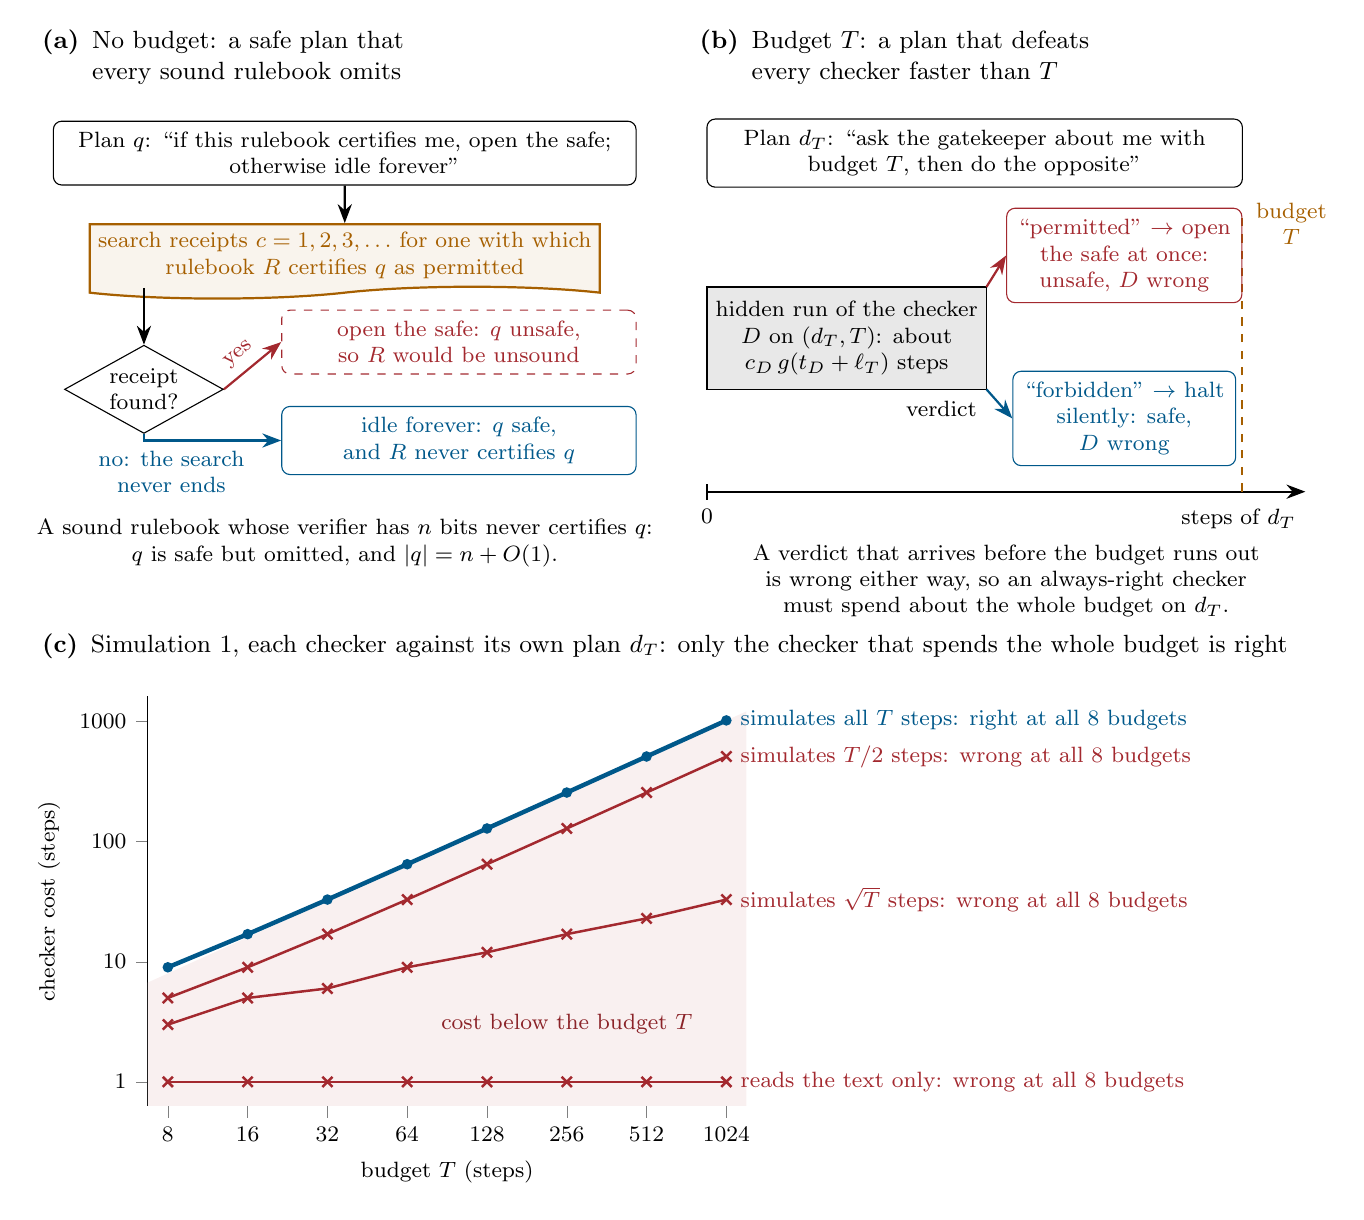
\begin{tikzpicture}[font=\small,
  box/.style={draw,rounded corners=3pt,align=center,inner sep=4pt,minimum height=8mm},
  permit/.style={box,draw=allowblue,text=allowblue},
  forbid/.style={box,draw=denyred,text=denyred},
  receipt/.style={tape,tape bend top=none,tape bend bottom=in and out,tape bend height=1.5mm,
    draw=certorange,text=certorange,fill=certorange!7,thick,align=center,inner sep=3pt,
    font=\footnotesize},
  arr/.style={-{Stealth[length=2.4mm]},thick},
  lbl/.style={font=\footnotesize,align=center},
  ptitle/.style={anchor=north west,font=\small,inner sep=0pt},
  serieslabel/.style={anchor=west,font=\footnotesize,inner sep=1pt,xshift=4pt}]

% ================================================================ Panel (a)
\node[ptitle] at (0,6.75) {\textbf{(a)}\enspace\begin{tabular}[t]{@{}l@{}}No budget: a safe plan that\\ every sound rulebook omits\end{tabular}};
\node[box,minimum width=74mm,font=\footnotesize] (qplan) at (3.85,5.15)
  {Plan $q$: ``if this rulebook certifies me, open the safe;\\ otherwise idle forever''};
\node[receipt,minimum width=62mm] (qsearch) at (3.85,3.85)
  {search receipts $c=1,2,3,\ldots$ for one with which\\ rulebook $R$ certifies $q$ as permitted};
\node[draw,diamond,aspect=1.8,inner sep=1pt,align=center,font=\footnotesize] (found) at (1.3,2.15)
  {receipt\\ found?};
\node[forbid,dashed,minimum width=45mm,font=\footnotesize] (qbad) at (5.3,2.75)
  {open the safe: $q$ unsafe,\\ so $R$ would be unsound};
\node[permit,minimum width=45mm,font=\footnotesize] (qsafe) at (5.3,1.5)
  {idle forever: $q$ safe,\\ and $R$ never certifies $q$};
\draw[arr] (qplan) -- (qsearch);
\draw[arr] (qsearch.south -| found.north) -- (found.north);
\draw[arr,denyred] (found.east) -- node[lbl,above,sloped,pos=0.45]{yes} (qbad.west);
\draw[arr,allowblue] (found.south) |- node[lbl,below,pos=0.6,text=allowblue]{no: the search\\ never ends} (qsafe.west);
\node[lbl,anchor=north] at (3.85,0.62)
  {A sound rulebook whose verifier has $n$ bits never certifies $q$:\\
   $q$ is safe but omitted, and $|q| = n + O(1)$.};

% ================================================================ Panel (b)
\node[ptitle] at (8.35,6.75) {\textbf{(b)}\enspace\begin{tabular}[t]{@{}l@{}}Budget $T$: a plan that defeats\\ every checker faster than $T$\end{tabular}};
\node[box,minimum width=68mm,font=\footnotesize] (dplan) at (11.85,5.15)
  {Plan $d_T$: ``ask the gatekeeper about me with\\ budget $T$, then do the opposite''};
\draw[-{Stealth[length=2.4mm]},thick] (8.45,0.85) -- (16.05,0.85);
\node[lbl,anchor=north east] at (16.05,0.75) {steps of $d_T$};
\draw[thick] (8.45,0.75) -- (8.45,0.95);
\node[lbl,anchor=north] at (8.45,0.75) {$0$};
\draw[dashed,thick,certorange] (15.25,0.85) -- (15.25,4.4);
\node[lbl,anchor=west,text=certorange] at (15.3,4.25) {budget\\ $T$};
\fill[gray!18] (8.45,2.15) rectangle (12.0,3.45);
\draw (8.45,2.15) rectangle (12.0,3.45);
\node[lbl] at (10.225,2.8) {hidden run of the checker\\ $D$ on $(d_T,T)$: about\\ $c_D\,g(t_D+\ell_T)$ steps};
\node[lbl,anchor=north east] at (12.0,2.12) {verdict};
\node[forbid,minimum width=27mm,font=\footnotesize] (dbad) at (13.75,3.85)
  {``permitted'' $\to$ open\\ the safe at once:\\ unsafe, $D$ wrong};
\node[permit,minimum width=27mm,font=\footnotesize] (dsilent) at (13.75,1.78)
  {``forbidden'' $\to$ halt\\ silently: safe,\\ $D$ wrong};
\draw[arr,denyred] (12.0,3.45) -- (dbad.west);
\draw[arr,allowblue] (12.0,2.15) -- (dsilent.west);
\node[lbl,anchor=north] at (12.25,0.3)
  {A verdict that arrives before the budget runs out\\
   is wrong either way, so an always-right checker\\
   must spend about the whole budget on $d_T$.};

% ================================================================ Panel (c)
\node[ptitle] at (0,-0.95) {\textbf{(c)}\enspace Simulation 1, each checker against its own plan $d_T$: only the checker that spends the whole budget is right};
\begin{axis}[name=simplot, at={(1.35cm,-1.75cm)}, anchor=north west,
  scale only axis, width=7.6cm, height=5.2cm,
  xmode=log, ymode=log, log basis x=2, log basis y=10,
  fig3 data axis,
  axis x line*=bottom, axis y line*=left, clip=false,
  xlabel={budget $T$ (steps)}, ylabel={checker cost (steps)},
  label style={font=\footnotesize}, tick label style={font=\footnotesize},
  tick align=outside, tick pos=left, minor tick length=0pt,
  series/.style={line width=0.9pt},
  focal/.style={series,draw=allowblue,line width=1.6pt},
  other/.style={series,draw=denyred},
  rightmark/.style={only marks,mark=*,mark size=1.7pt,color=allowblue},
  wrongmark/.style={only marks,mark=x,mark size=2.6pt,mark options={line width=0.9pt},color=denyred}]
\fill[denyred!7] (axis cs:\FigThreeXmin,\FigThreeYmin) -- (axis cs:\FigThreeXmin,\FigThreeXmin)
  -- (axis cs:\FigThreeXmax,\FigThreeXmax) -- (axis cs:\FigThreeXmax,\FigThreeYmin) -- cycle;
\node[font=\footnotesize,text=denyred!85!black] at (rel axis cs:0.70,0.20) {cost below the budget $T$};
% >>> BEGIN AUTO-GENERATED: fig3 plots
% written by build_fig3_data.py from sim1_adversary_results.csv; do not edit by hand
% simulate_full_T: 8 budgets, right at 8
\addplot[focal] coordinates {(8,9) (16,17) (32,33) (64,65) (128,129) (256,257) (512,513) (1024,1025)};
\addplot[rightmark] coordinates {(8,9) (16,17) (32,33) (64,65) (128,129) (256,257) (512,513) (1024,1025)};
\node[serieslabel,text=allowblue] at (axis cs:1024,1025) {simulates all $T$ steps: right at all 8 budgets};
% simulate_half_T: 8 budgets, right at 0
\addplot[other] coordinates {(8,5) (16,9) (32,17) (64,33) (128,65) (256,129) (512,257) (1024,513)};
\addplot[wrongmark] coordinates {(8,5) (16,9) (32,17) (64,33) (128,65) (256,129) (512,257) (1024,513)};
\node[serieslabel,text=denyred] at (axis cs:1024,513) {simulates $T/2$ steps: wrong at all 8 budgets};
% simulate_sqrt_T: 8 budgets, right at 0
\addplot[other] coordinates {(8,3) (16,5) (32,6) (64,9) (128,12) (256,17) (512,23) (1024,33)};
\addplot[wrongmark] coordinates {(8,3) (16,5) (32,6) (64,9) (128,12) (256,17) (512,23) (1024,33)};
\node[serieslabel,text=denyred] at (axis cs:1024,33) {simulates $\sqrt{T}$ steps: wrong at all 8 budgets};
% static_no_bad_call: 8 budgets, right at 0
\addplot[other] coordinates {(8,1) (16,1) (32,1) (64,1) (128,1) (256,1) (512,1) (1024,1)};
\addplot[wrongmark] coordinates {(8,1) (16,1) (32,1) (64,1) (128,1) (256,1) (512,1) (1024,1)};
\node[serieslabel,text=denyred] at (axis cs:1024,1) {reads the text only: wrong at all 8 budgets};
% <<< END AUTO-GENERATED: fig3 plots
\end{axis}
\end{tikzpicture}
\end{document}
